% Chapter Template

\chapter{Ordonnanceur} % Main chapter title

\label{Chapitre 3} % Change X to a consecutive number; for referencing this chapter elsewhere, use \ref{ChapterX}

\lhead{ \emph{Ordonnancement de tâches}} % Change X to a consecutive number; this is for the header on each page - perhaps a shortened title

Ce deuxième chapitre nous explique par l'exemple un peu l'ordonnancement des différentes tâches. Pour cela, nous allons utiliser une simple petite application qui va nous permettre d'essayer divers essais d'ordonnancement.

%----------------------------------------------------------------------------------------
%	SECTION 1
%----------------------------------------------------------------------------------------
\section{Exemple d'application}

Comme vous le savez, il y a deux types de ressources consommables :
\begin{itemize}
\item Consommation d'I/Os (Disque dur, port série, etc...)
\item Consommation en calculs (CPU)
\end{itemize}

Le but serait d'utiliser un peu les deux,afin d'observer les comportements possibles en exécution. Pour commencer, nous allons générer du temps de calcul, avec un exemple de programme qui calcule des nombres premiers. Voici le code :

\begin{lstlisting}[frame=single,style=C]  % Start your code-block

int prime_generation(long int aMaxNum) {
	int probe;
	int divisor;
	char primeNum;
	for (probe = 1; probe <= aMaxNum; probe++) {

		primeNum = 1; /* On image que le nombre est prime */

		for (divisor = 2; divisor < probe; divisor++) {
			if (probe % divisor == 0)
				primeNum = 0;
		}

	}
	return 0;
}
\end{lstlisting}


\pagebreak Comme ce bout de code n'est pas très optimisé pour la mesure, nous avons créé une nouvelle fonction plus adaptée. En voici le code :

\begin{lstlisting}[frame=single,style=C]  % Start your code-block

int prime_optimized(long int aMaxNum) {
	register int probe;
	register char primeNum;
	int lastPrimes[aMaxNum];
	register int nbPrimes = 0;
	register int i;
	for (probe = 2; probe <= aMaxNum; probe++) {

		primeNum = 1; /* On image que le nombre est prime */

		for (i = 0; i < nbPrimes; i++) {
			if (probe % lastPrimes[i] == 0) {
				primeNum = 0;
				break;
			}
		}

		/* output of the number ? */
		if (primeNum) {
			//printf("%8d\n", probe);
			lastPrimes[nbPrimes] = probe;
			nbPrimes++;
		}
	}
	return 0;
}
\end{lstlisting} 
 
Afin de pouvoir effectuer des mesures sans que la mesure même induise une erreur, nous effectuons l'appel de cette fonction plusieurs fois. Voici l'exemple de cette application :

\begin{lstlisting}[frame=single,style=C]  % Start your code-block

/* # of Numbers to test */
#define ITER_NUM	50
#define MAX_NUMBER 	1000

int main(){
...
	clock_gettime(CLOCK_REALTIME, &rt_start);

	// Faire quelques iterations pour que clock_gettime() n'aie
	// pas trop d'influence
	for (i = 0; i < ITER_NUM; i++) {

		// Fonction à tester 1
		//With 1000 optimised
		//prime_generation(MAX_NUMBER);
		prime_optimized(MAX_NUMBER);
		//prime_fileWrite(MAX_NUMBER);
		//prime_Write(MAX_NUMBER);

	}

	clock_gettime(CLOCK_REALTIME, &rt_stop);
...
}
\end{lstlisting} 

\pagebreak \section{Priorité des tâches}

A chaque processus est associé une politique d'ordonnancement et une priorité statique (qui dépend de la politique d'ordonnancement). Pour les processus qui utilisent la politique d'ordonnancement standard, leur priorité statique est calculé 120 + valeur nice. 

Cette dernière peut être changée avec la commande "nice". Cette commande peut recevoir des valeur entre -20 et 19 (nouvelle priorité), -20 étant la plus priorité la plus grande (cette valeur influence le "timeslice" alloué à celle-ci). Nous y reviendrons plus tard.

Voici une petite illustration de ces priorités :\\

\textbf{HIGH PRIORITY----------------------------------------------------------------LEAST PRIORITY}\\
-------------------------------------------------------------------------------------------------------------------------------\\
99 ........................... 50 .......................... 1 | -20 ............. -10 ............ 0 ............. 10 ............. 19\\
-------------------------------------------------------------------------------------------------------------------------------\\

Vous pouvez constater que les nombre sont séparé en 2 par le caractère "|". Les priorités de 99 à 1 sont réservé pour les processus qui on des contraintes de temps (SCHED\_FIFO, SCHED\_RR). Les priorités de 100 à 139 sont réservé aux processus normaux (SCHED\_OTHER). Pour mieux comprendre il faut que nous nous intéressions aux différentes politique d'ordonnancement. 

\section{Scheduler policy}

Sous Linux, il y a 3 différentes politique d'ordonnancement. En voici une liste :
\begin{itemize}
\item \textbf{SCHED\_FIFO} : 
\item \textbf{SCHED\_RR} :
\item \textbf{SCHED\_OTHER} : SAlut\\
\end{itemize}

Sans spécification de politique d'ordonnancement, les processus possède la politique SCHED\_OTHER et une priorité statique de 0. La priorité change dynamiquement suivant l'évolution de l'exécution des différentes tâches. Cette priorité peut être influencé par la valeur de "nice" qui peut varier de -20 à 19. On peut notamment la spécifier grâce à la commande "nice". Voilà un illustration graphique de notre application exécutée avec différente valeur de "nice" :

\begin{center} 
\hspace{12.45cm}
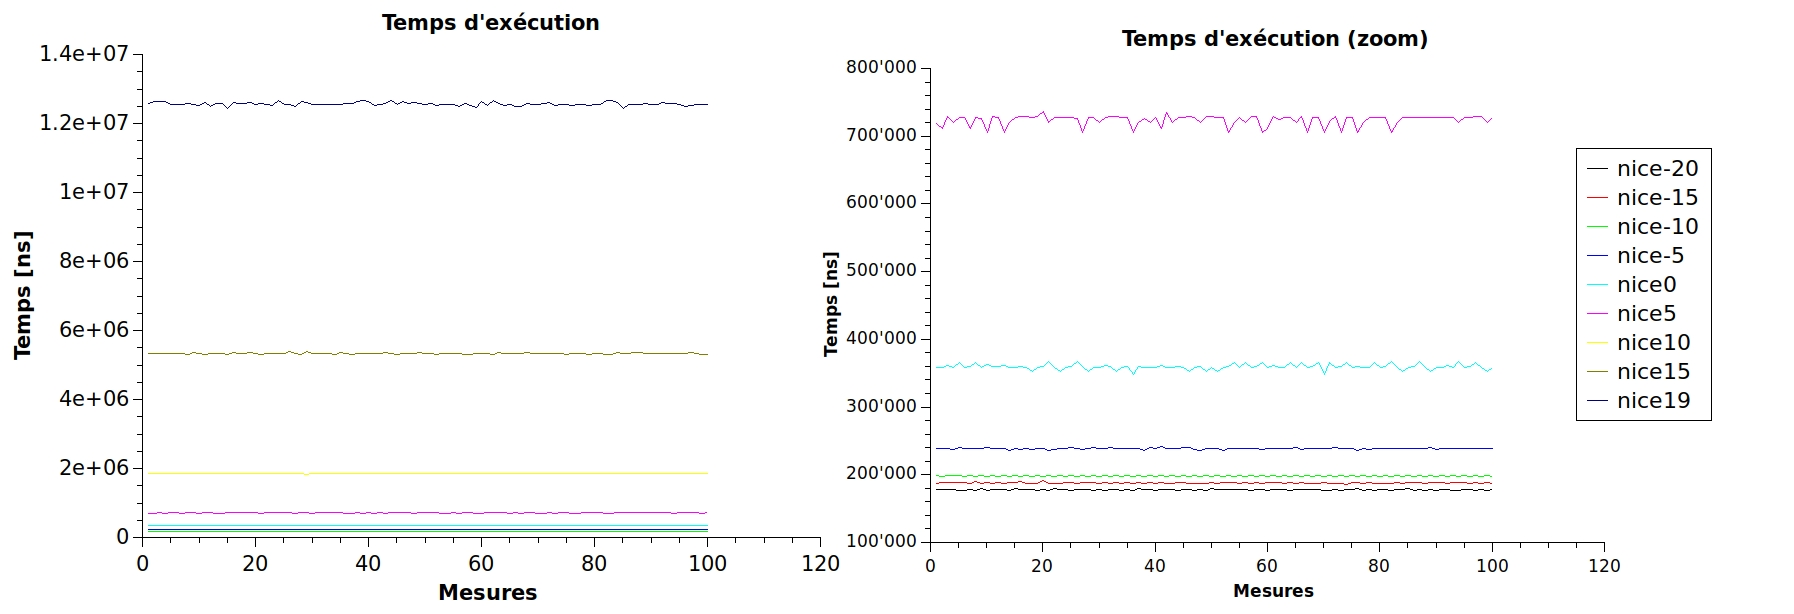
\includegraphics[width=19cm]{Nice_Moyenne.jpg}
\end{center}
\vspace{1cm}

On peut voir le temps d'exécution de la fonction de calcul suivant les différentes valeur de "nice". Le graphique de droite est un zoom sur les courbes situé en bas du graphique de gauche. On peut s'intéresser maintenant à la répartition statistique de ces valeurs moyenne. Voici un histogramme pour différentes valeur de "nice" :

\begin{center} 
\hspace{12.45cm}
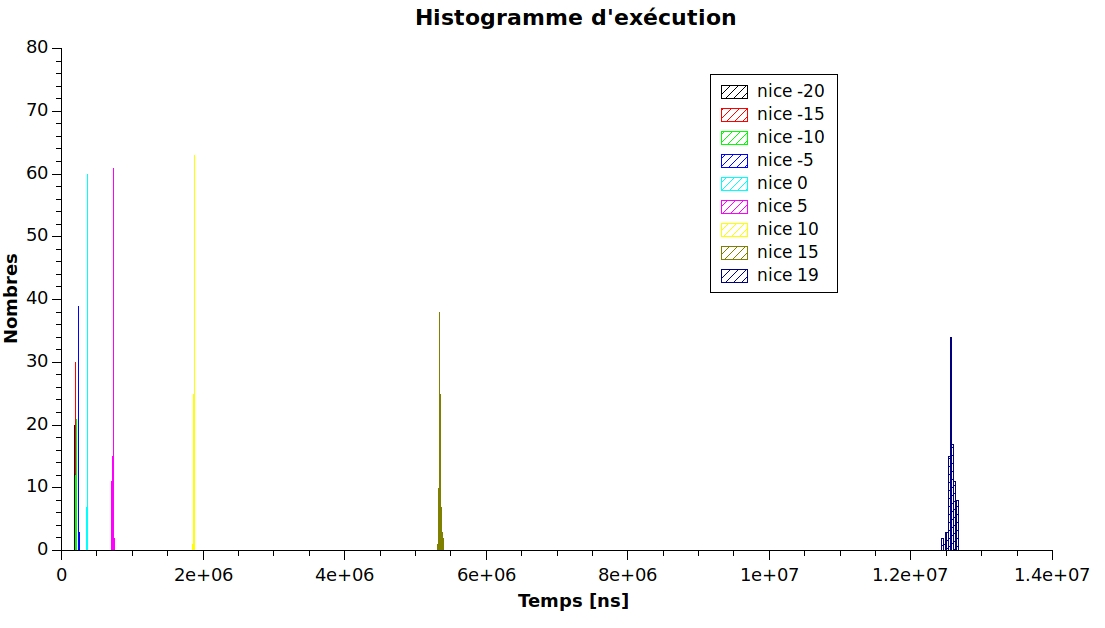
\includegraphics[width=17cm]{Hist_Nice.jpg}
\end{center}
\vspace{1cm}

On peut imaginer une sorte de gaussienne. Voici un zoom sur l'histogramme le plus à gauche :

\begin{center} 
\hspace{12.45cm}
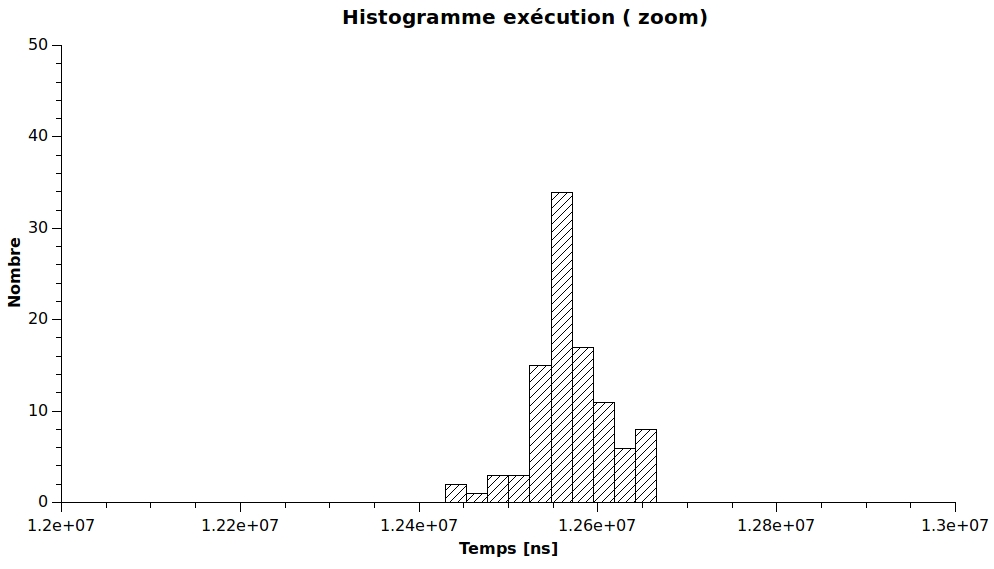
\includegraphics[width=17cm]{Hist_Nice_zoom.jpg}
\end{center}
\vspace{1cm}

On observe bien une courbe de gauss sur le temps d'exécution des différentes tâches. Ce qui pourrait être intéressant, ce serait d'observer le temps d'exécution de la fonction lorsque le système est en charge. Donc lançons l'exécution de notre tâche sur un système en charge avec "N" processus, sans spécification d'ordonnancement (SCHED\_OTHER)\footnote{La commande "chrt" sous Linux permet de connaître la politique d'ordonnancement actuelle d'un processus.}. Voici le résultat moyen :
 
\begin{center} 
\hspace{12.45cm}
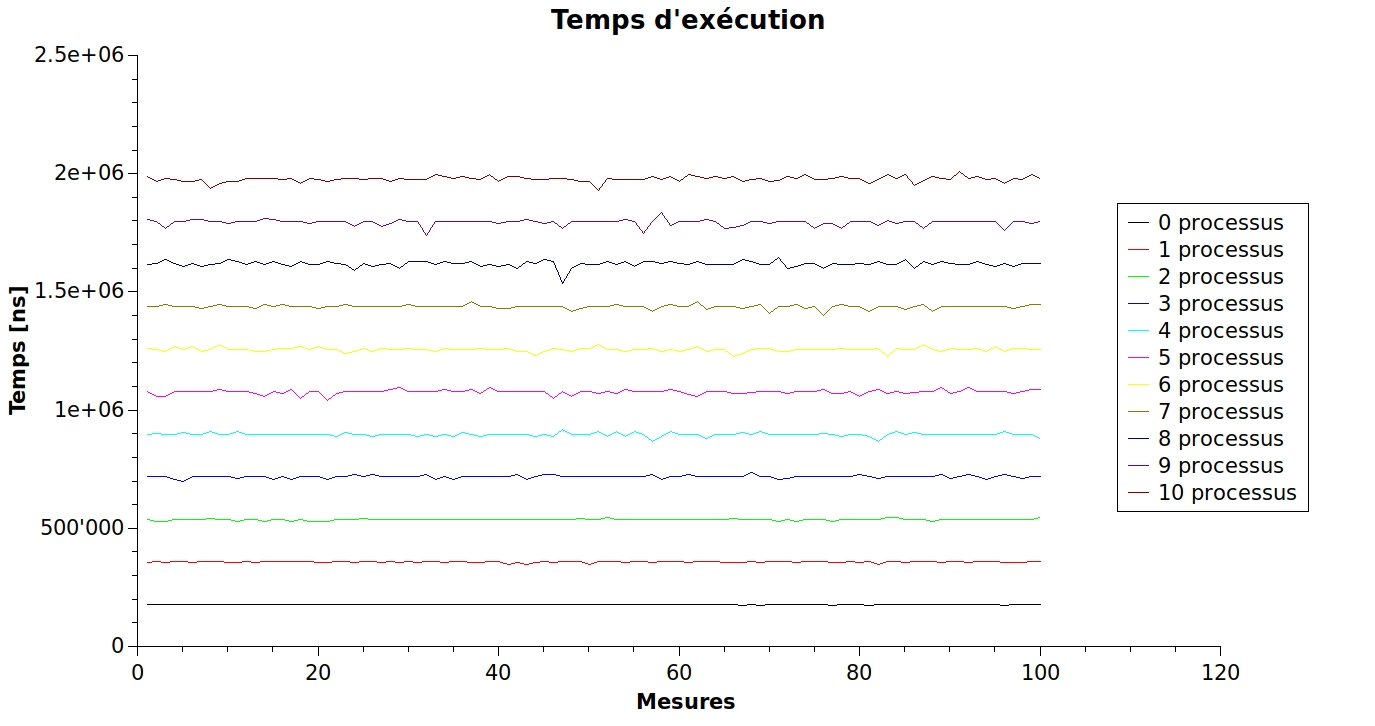
\includegraphics[width=17cm]{NProc_All.jpg}
\end{center}
\vspace{0.5cm}

Les processus concurrent sont la commande "yes" lancée plusieurs fois:
\begin{lstlisting}[frame=single,style=Console]  % Start your code-block

$ yes > /dev/null &
\end{lstlisting}

Les espaces entre les courbes ont l'air réguliers ! Essayons de tracer le temps d'exécution en fonction des processus. Voici le graphique de cette représentation :
 
\begin{center} 
\hspace{12.45cm}
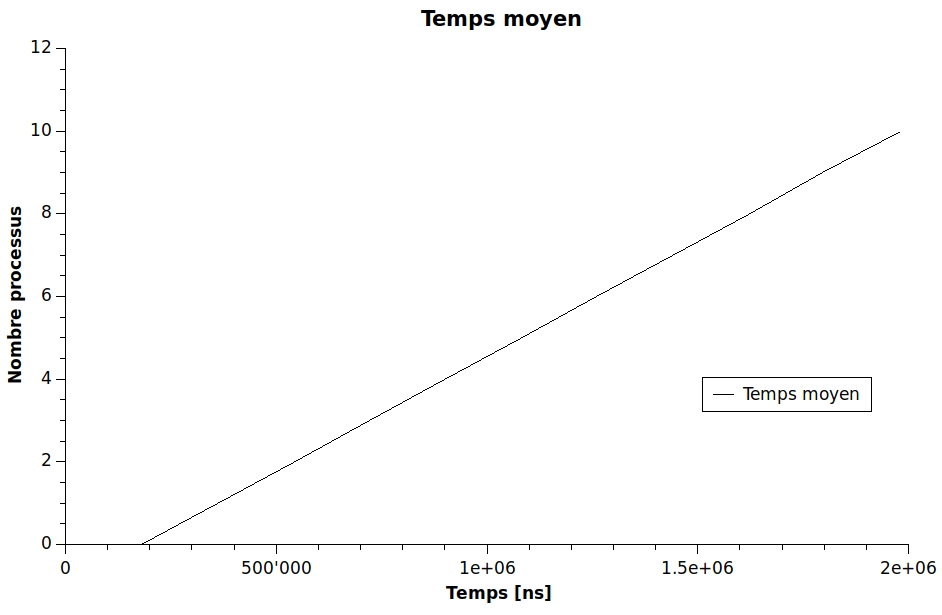
\includegraphics[width=12.5cm]{NProc_Moy.jpg}
\end{center}
\vspace{1cm}

\pagebreak On voit que c'est parfaitement linaire. On peut essayer de vérifier maintenant le si la politique d'ordonnancement normale est bien SCHED\_OTHER. Voici la courbe de moyennes :

\begin{center} 
\hspace{12.45cm}
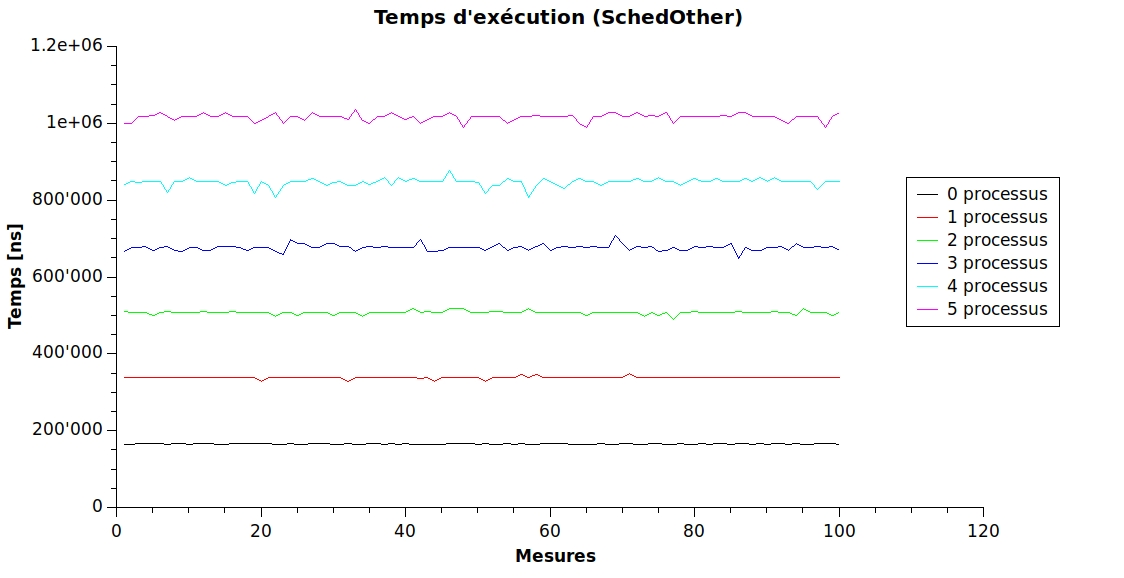
\includegraphics[width=18cm]{SChedOther_ALL.jpg}
\end{center}
\vspace{1cm}

Ainsi que l'autre représentation (nombre de processus et temps d'exécution) :

\begin{center} 
\hspace{12.45cm}
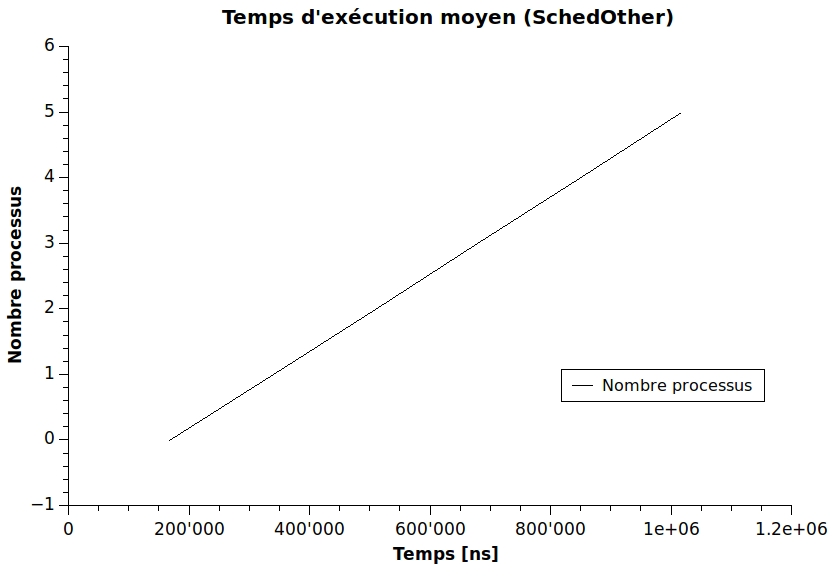
\includegraphics[width=15cm]{SChedOther_Moy.jpg}
\end{center}
\vspace{1cm}

\pagebreak C'est exactement le même comportement que le précédent. On peut donc en conclure que la politique d'ordonnancement de base est SCHED\_OTHER ! Essayons maintenant de changer la politique en SCHED\_FIFO. Voilà le résultat pour une priorité de 1, 50, \textbf{100} :

\begin{center} 
\hspace{12.45cm}
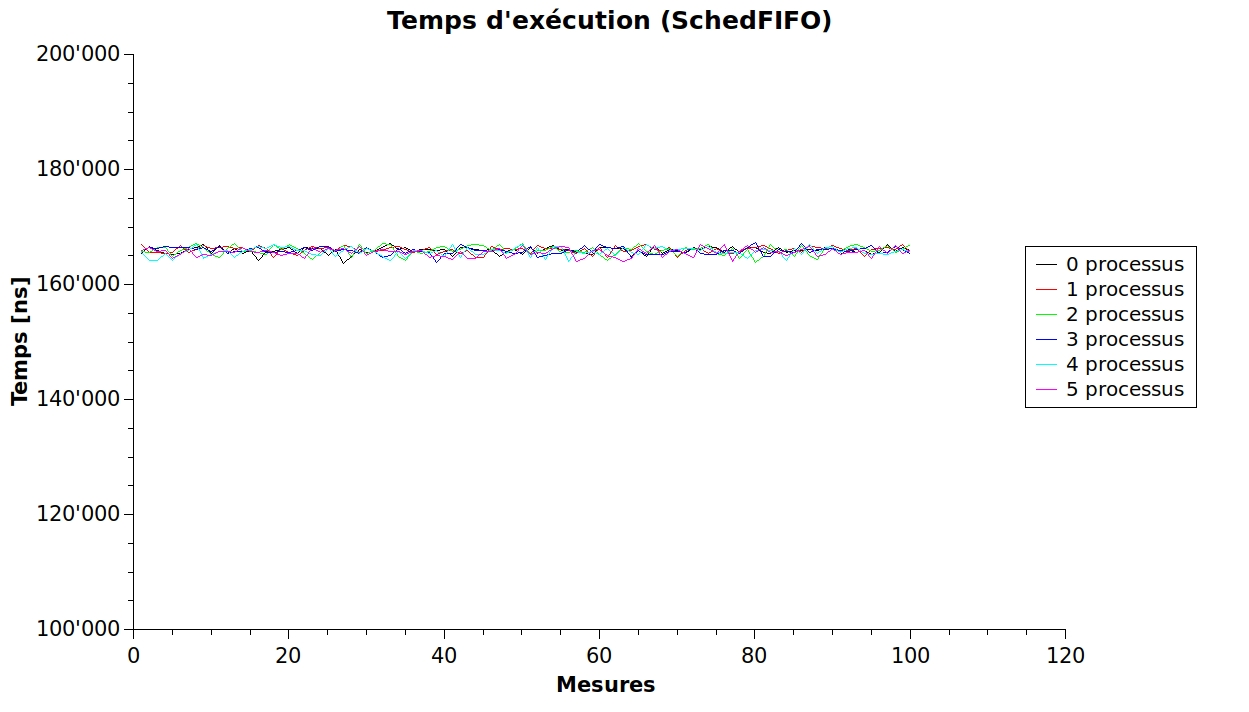
\includegraphics[width=17cm]{SchedFIFO_p1.jpg}
\end{center}
\vspace{0.5cm}

\begin{center} 
\hspace{12.45cm}
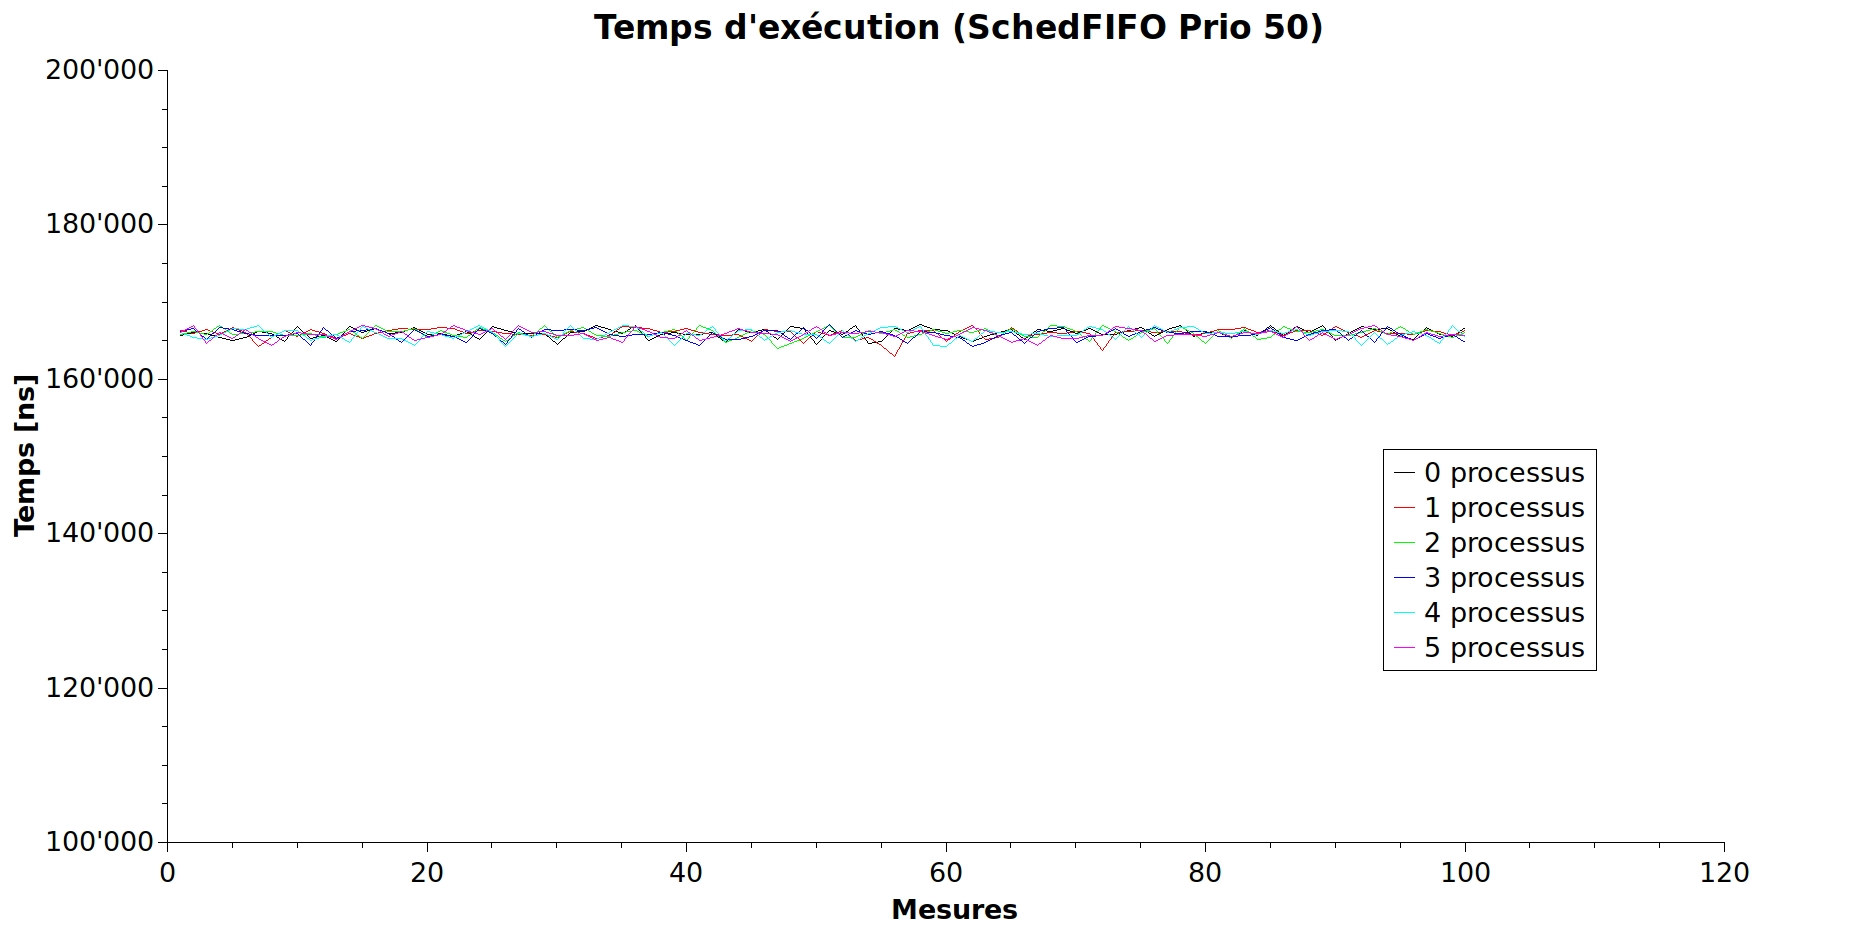
\includegraphics[width=17cm]{SchedFIFO_p50.jpg}
\end{center}
\vspace{0.5cm}

\begin{center} 
\hspace{12.45cm}
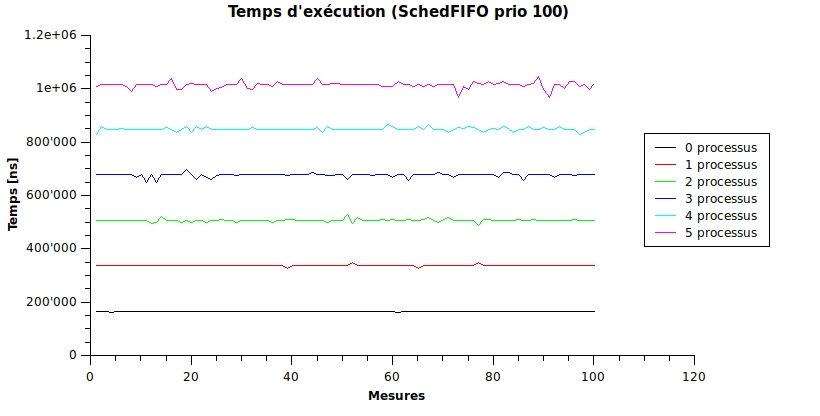
\includegraphics[width=17cm]{SchedFIFO_p100.jpg}
\end{center}
\vspace{0.5cm}

Constatations : Pour les priorités 1 et 50, le temps d'exécution de la tâche ne varie pratiquement pas ! Par contre pourquoi avec 100 on obtient un comportement bizzare ? \\

La fonction "\textbf{sched\_setscheduler()}" donne une valeur de retour que nous n'avions pas testée... Ce qui signifie que la priorité 100 n'existe pas car la "priorité" maximum est de 99. Le résultat est que l'application a fonctionné en politique normale ! (Nous n'avons pas eu le temps de refaire les mesures, désolé...)\\

Ce que nous aurions pu encore faire, est de lancer plusieurs fois notre tâche et de voir si le système se comporte bien en FIFO (ce serait été le but).

\pagebreak Essayons de refaire exactement les mêmes essais qu'avec la politique SCHED\_FIFO, mais pour SCHED\_RR. Voici les graphiques correspondants :

\begin{center} 
\hspace{12.45cm}
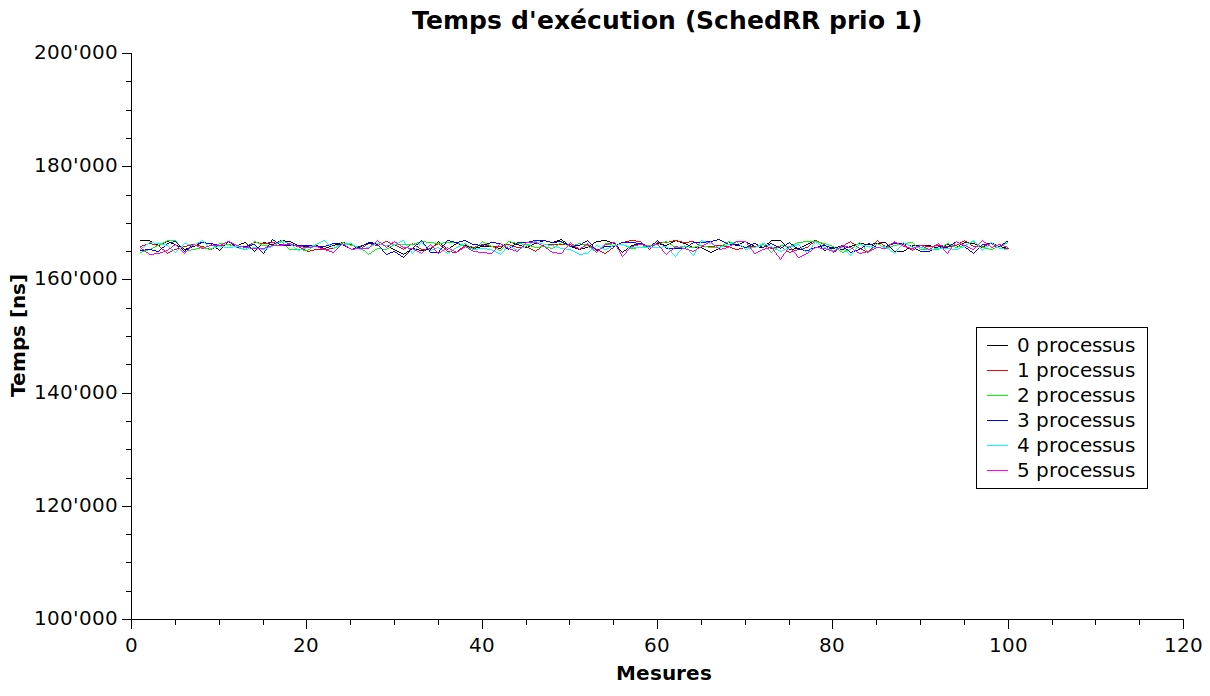
\includegraphics[width=17cm]{SchedRR_p1.jpg}
\end{center}
\vspace{0.5cm}

\begin{center} 
\hspace{12.45cm}
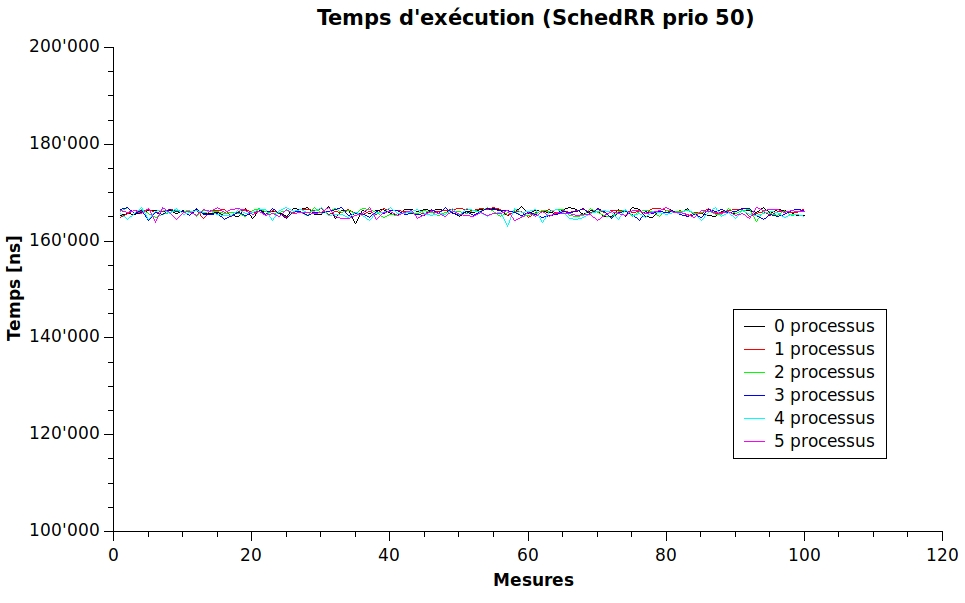
\includegraphics[width=17cm]{SchedRR_p50.jpg}
\end{center}
\vspace{0.5cm}

\begin{center} 
\hspace{12.45cm}
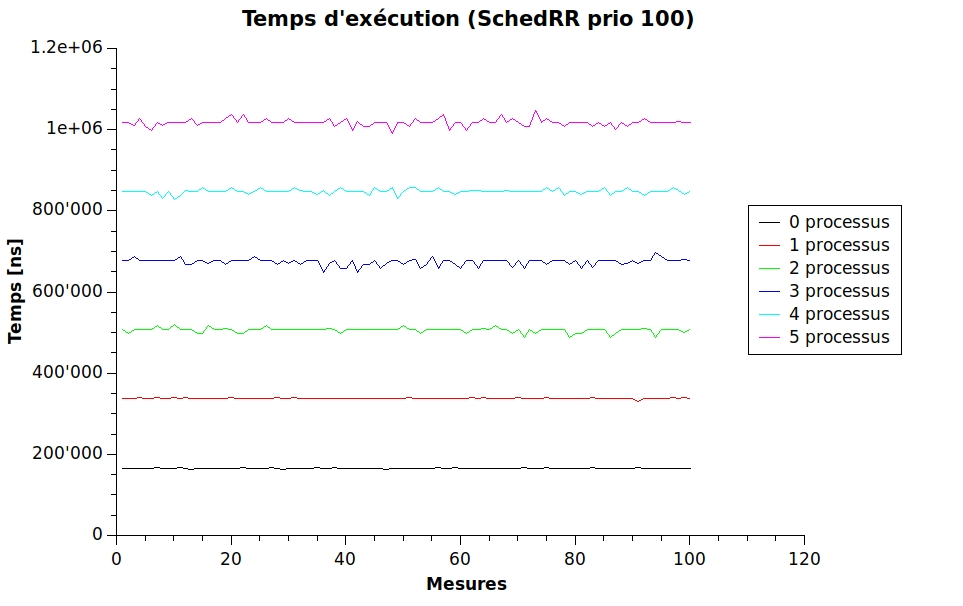
\includegraphics[width=17cm]{SchedRR_p100.jpg}
\end{center}
\vspace{0.5cm}

On peut faire exactement les mêmes constations qu'avec les mesures précédentes :
\begin{itemize}
\item Le priorité 100 n'existe pas (maximum 99).
\item Nous aurions pu lancer plusieurs fois la tâche en parallèle pour vérifier le bon fonctionnement de la politique d'ordonnancement.\\
\end{itemize} 

Par contre, on remarque que le temps d'exécution moyen de la tâche (par rapport à une politique SCHED\_OTHER) est égale à celui le plus bas (~165000 ns)! 

Donc pour des tâches ayant des contrainte de temps, il vaudrait mieux utiliser les politique d'ordonnancement SCHED\_RR ou SCHED\_FIFO.


\pagebreak \section{La hiérarchie Cgroups}

Ce qui pourrait nous intéresser maintenant, c'est de pouvoir réserver ou de partager de manière fixe les ressource du processeur (temps de calcul, I/Os). Imaginons qu'un serveur web soit attaqué et que le processeur soit tellement chargé que l'on ne puisse même pas atteindre la ligne de commande\footnote{Exemple cité en cours} ! \\

Pour contrer à ce problème, le noyau Linux nous met un outils à disposition pour allouer un certains nombre de ressources à un groupe défini : \textbf{la hiérarchie Cgroups}. Afin de pourvoir l'essayer, imaginons le même scénario qu'avant, mais cette fois on alloue statiquement les ressources pour notre application et pour les processus en charge. C'est à dire, par exemple 5\% pour les processus de charge et 95\% pour notre application.\\

Pour l'utiliser les "cgroups", il ne faut pas oublier de les activer dans le noyau (configuration et compilation nécessaire). Une fois fait, on peut monter la hierarchie cgroups sur notre système de fichier avec la commande suivante :

\begin{lstlisting}[frame=single,style=Console]  % Start your code-block

$ mount -t cgroup -o cpu groups /cgroups
\end{lstlisting}

Cela va monter cette fameuse "parition" cgroups. Créeons maintenant un sous-dossier qui contiendra le partage pour notre application et un autre pour les autres processus :

\begin{lstlisting}[frame=single,style=Console]  % Start your code-block

$ mkdir /cgroups/program
$ mkdir /cgroups/low
\end{lstlisting}

Et ensuite on peut mettre la proportion que l'on veut donner à chaqu'un des sous-groupes ("program" et "low") :

\begin{lstlisting}[frame=single,style=Console]  % Start your code-block

$ echo 1024 > /cgroups/program/cpu.shares
$ echo 1024 > /cgroups/low/cpu.shares
\end{lstlisting}

Si on veut allouer moins de ressources à notre application :
\begin{lstlisting}[frame=single,style=Console]  % Start your code-block

$ echo 102 > /cgroups/program/cpu.shares
\end{lstlisting}

Et plus pour les autre applications :
\begin{lstlisting}[frame=single,style=Console]  % Start your code-block

$ echo 1946 > /cgroups/low/cpu.shares
\end{lstlisting}

Remarque : la somme des "cpu.shares" doit être égal à 2048. On peut calculer le pourcentage réservé à chacun pour la configuration que l'on vient d'effectuer :\\

\begin{align*}
Low_\% &= \frac{1946}{2048} \cdot 100 \approx 95\%  \\
App_\% &= \frac{102}{2048} \cdot 100 \approx 5\%
\end{align*}



\pagebreak Voilà ce que donne le temps d'exécution pour divers valeur alloué pour notre tâche (5\%, 50\% et 95\%) :

\begin{center} 
\hspace{12.45cm}
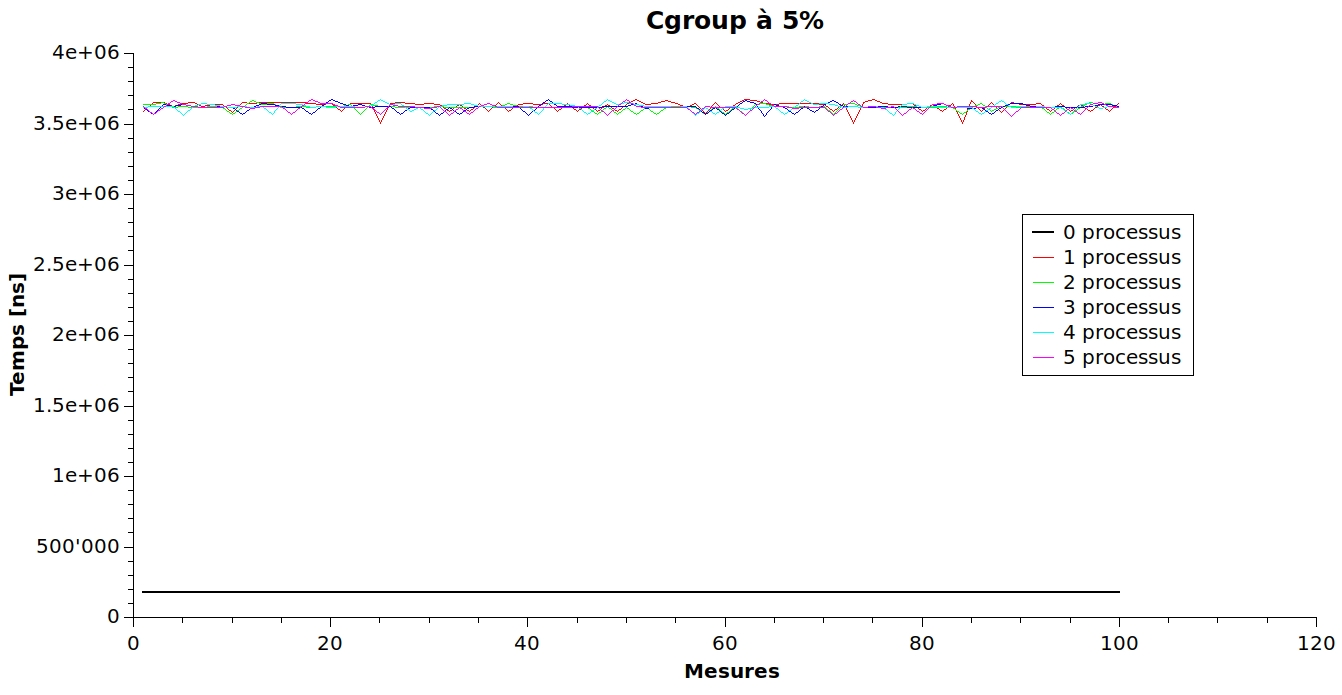
\includegraphics[width=17cm]{Cgoup5.jpg}
\end{center}
\vspace{1cm}


\begin{center} 
\hspace{12.45cm}
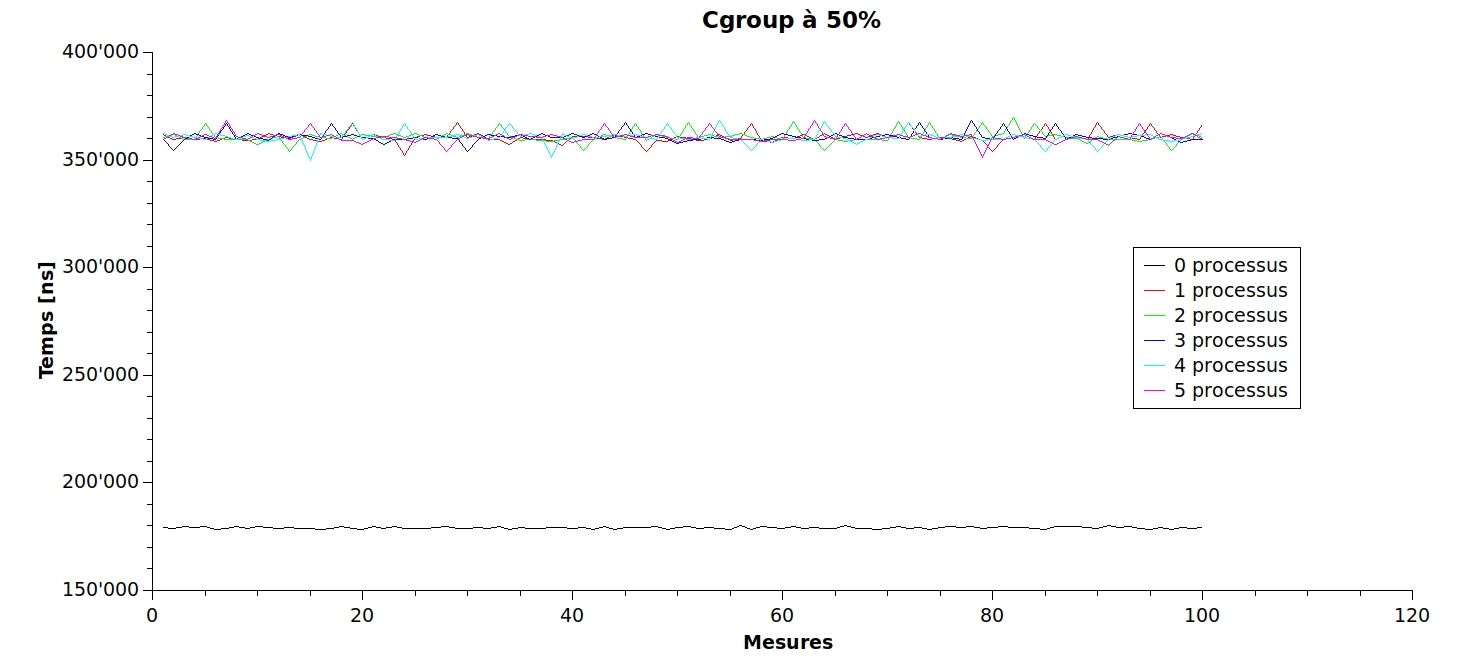
\includegraphics[width=18cm]{Cgoup50.jpg}
\end{center}
\vspace{0.5cm}


\begin{center} 
\hspace{12.45cm}
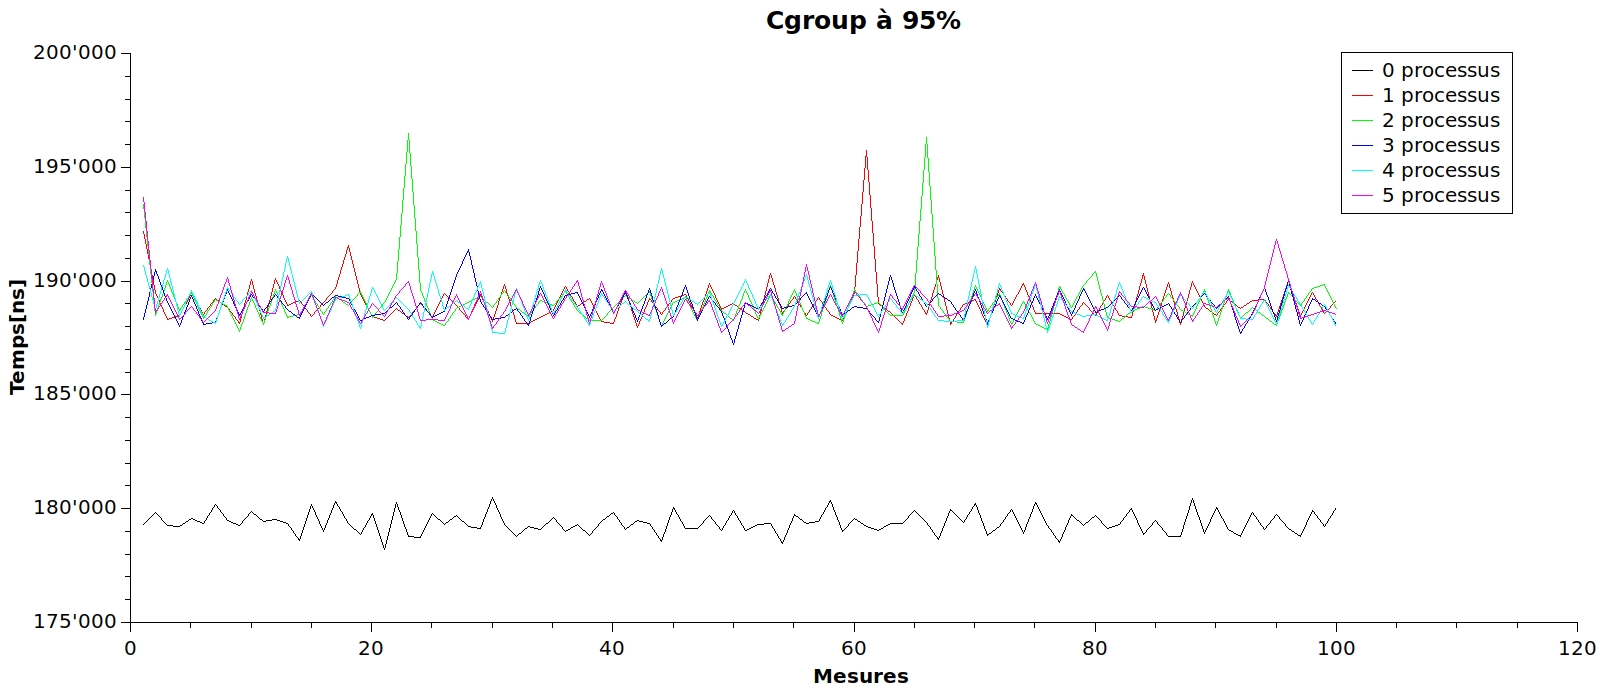
\includegraphics[width=17cm]{Cgoup95.jpg}
\end{center}
\vspace{0.5cm}

 

On voit aisément que plus on alloue de ressource à notre application, plus la différence de temps d'exécution à 0 processus et à N processus devient faible. De plus, on peut voir que si le système est chargé à 1 ou à N processus, cela ne change "rien" au temps d'exécution de la tâche.\\

Pour conclure cette partie du chapitre, nous avons aussi effectué d'autres essais (c.f. code source) avec une fonction qui écrit les nombre premier calculé dans un fichier, donc qui utilise des I/Os. Le temps nous a manqué pour approfondir les mesures, mais ce serait intéressant de voir les différences. De plus, nous avons implémenté deux fonctions qui utilise des I/Os différemment : une fois la fonction écrit à chaque fois ("write()") et bloque, ensuite une autre qui utilise un tampon pour les données et écrit ensuite un grand paquet ("fwrite()").\\

Petite anecdote à ce sujet : au cours d'ICR (Industrial Cryptography), nous avons du implémenter un système qui permet de créer un container sécurisé. Une fois nous avons utilisé la fonction "write()" et ensuite changé en "fwrite()" (les blocs écrit sont de taille 16 bytes pour un chiffrement symétrique AES) . Dans le premier cas, la phase de chiffrement prenait 70 seconde, et dans le second 5 secondes ! La performance est nettement améliorée uniquement en ajoutant une lettre à la fonction (hahahaha...)!

